% DIAGNOSTICS
% Author:
% March 2008, J.-P. Chaboureau, editorial corrections
%%%%%%%%%%%%%%%%%%%%%%%%%%%%%%%%%%%%%%%%%%%%%%%%%%%%%%%%%%%%%%%%%%%%%%%%%%%%%%%
\chapter{Diagnostics}
\minitoc


\section{Some formulae}

\subsubsection{Temperature}
The temperature {\tt TEMP} ($^\circ$C) is computed as:
\begin{equation}
T = \Pi \theta - T_t
\end{equation}
where $T_t$ is the temperature of the triple point.


\subsubsection{Vapor pressure  and  relative humidity}
The vapor pressure ({\tt VPRES}) is computed as:
\begin{equation}
e = \dfrac{P}{1 + r_v \, R_d/R_v} 
\end{equation}
The relative humidity ({\tt REHU}) is computed as:
\begin{eqnarray}
Hu &=& \dfrac{e}{e_s(T)} 
\end{eqnarray}
When a mixed microphysical scheme is activated during the simulation,
 the saturation vapor pressure $e_s(T)$ is computed over ice
 at points where temperature is below the triple point.
 

\subsubsection{Refraction coindexes}
Following \citet{Hill1980} the refraction coindex ({\tt COREF}) is computed as:
\begin{equation}
  N = (77.6/T)\times(P+4810\,e/T) -6e/T
\end{equation}
where $P$ and $e$ are in hPa.

\noindent The modified refraction coindex ({\tt MCOREF}) is computed as:
\begin{equation}
  M = N + Z\,10^6 a
\end{equation}
where $Z$ and $a$ are respectively the altitude and the Earth radius in m.


\subsubsection{Virtual potential temperature}
The virtual potential temperature ({\tt THETAV}) is given by:
\begin{eqnarray}
\theta_v &=& \theta \times \dfrac{(1 + r_v R_v /R_d)}
                            {(1+r_w)}
\end{eqnarray}
where $r_w$ is the mixing ratio of total water substance
\begin{eqnarray}
r_w &=& r_v+r_c+r_r+r_i+r_s+r_g+r_h   \nonumber
\end{eqnarray}


\subsubsection{Equivalent potential temperature}
The formulation of the equivalent potential temperature ({\tt THETAE})
is taken from \citet{Bolton1980} following its equations (16), (21) and (43):
\begin{eqnarray}
\theta_e &=& \theta \, \exp \left[\Big(\dfrac{3376}{T_L} - 2.54\Big) 
                    \, r_v \, (1 + 0.81 r_v) \right ] \\
\mbox{where } T_L &=& \dfrac{2840}{3.5 \ln T - \ln e - 4.805} +55 \nonumber \\
\mbox{ and } e   &=& \frac{0.01\, P \, r_v}{0.622 +r_v} \nonumber
\end{eqnarray}


\subsubsection{Vorticity quantities}
The relative vorticity ({\tt UM1,VM1,WM1}) is computed as:
\begin{eqnarray}
\vec\zeta= \vec{\nabla}\wedge\vec{U} &= &
(\dfrac{\partial w}{\partial\hat{y}} - \dfrac{\partial v}{\partial\hat{z}})\vec{i}
\nonumber \\
& &+ (\dfrac{\partial u}{\partial\hat{z}} - \dfrac{\partial w}{\partial\hat{x}})\vec{j}
\nonumber \\
& &+ (\dfrac{\partial v}{\partial\hat{x}} - \dfrac{\partial u}{\partial\hat{y}})\vec{k}
\end{eqnarray}
The absolute vorticity ({\tt ABVOR}) 
takes into account the rotation of the earth:
\begin{equation}
\xi= \vec{\zeta}.\vec{k} + 2 \Omega\sin\varphi
\end{equation}


\subsubsection{Potential vorticity}
The Ertel potential vorticity  ({\tt POVOM}) is computed as:
\begin{equation}
P = \dfrac{\vec\zeta .\vec\nabla(\theta)}{\rho_{dref}} 
\end{equation}
The unit is the Potentiel Vorticity Unit, 
$1$~PVU$=10^6$~K~m$^2$~kg$^{-1}$~s$^{-1}$


\subsubsection{Moist potential vorticities}
The virtual potential vorticity ({\tt POVOV}) is
\begin{equation}
P_v = \dfrac{\vec\zeta .\vec\nabla(\theta_v)}{\rho_{dref}} 
\end{equation}
and the equivalent virtual potential vorticity ({\tt POVOE}) 
\begin{equation}
P_e = \dfrac{\vec\zeta .\vec\nabla(\theta_e)}{\rho_{dref}} 
\end{equation}


\subsubsection{Geostrophic and ageostrophic winds}
With the LHE system (see Chapter Basic Equations in Part I), the geostrophic wind 
({\tt UM88,VM88, UM89,VM89}) is computed as:
\begin{eqnarray}
u_g= - \dfrac{1}{f}\,\dfrac{\partial{(C_{pd}\theta_{vref}\Pi^{'})}}{\partial\hat{y}} &;&
v_g=   \dfrac{1}{f}\, \dfrac{\partial{(C_{pd}\theta_{vref}\Pi^{'})}}{\partial\hat{x}} 
\end{eqnarray}

\noindent With the MAE and DUR systems (see book1, chapter 2), 
the geostrophic wind is computed as:
\begin{eqnarray}
u_g= - \dfrac{1}{f} \, C_{pd}\theta_{vref} \,
       \dfrac{\partial\Pi^{'}}{\partial\hat{y}} &;&
v_g=   \dfrac{1}{f} \, C_{pd}\theta_{vref} \,
       \dfrac{\partial\Pi^{'}}{\partial\hat{x}}
\end{eqnarray}
where $$
\Pi^{'} = \left(\dfrac{P}{P_{00}}\right)^{\frac{R_d}{C_{pd} }} - \Pi_{ref} $$

\noindent The ageostrophic wind is computed as: 
\begin{eqnarray}
u_{ag} = u - u_g &;& v_{ag} = v - v_g \nonumber
\end{eqnarray}
%
\subsubsection{Near-surface wind}
%
Zonal and meridional wind at 10\,m height above ground level (AGL), $u_\mathrm{10m}, v_\mathrm{10m}$ are stored in variables {\tt UM10}, {\tt VM10} and computed as:
\begin{itemize}
\item If {\tt IKB} = 1 + {\tt JPVEXT} (first physical vertical level) is above 10\,m height AGL: XCURRENT\_ZON10M and XCURRENT\_MER10M are initialized by
SURFEX model diagnostic variables {\tt ZON10M}, {\tt MER10M} and not equal to XUNDEF if {\tt N2M} > 0 in NAM\_DIAG\_SURFn.
%SURFEX routine "get\_fluxn.F90" computes PZON10M and PMER10M if N2M>0 in \&NAM\_DIAG\_SURFn and Meso-NH routines "mnhget\_surf\_paramn.f90" and "ground\_paramn.f90".
\begin{align}
u_\mathrm{10m} &= {\tt ZON10M}\\
v_\mathrm{10m} &= {\tt MER10M}
\end{align}
\item If {\tt IKB} is below 10\,m height AGL, then at the mass level $z_i = {\tt XZHATM}(i)$ at which ${\tt XZHATM}(i) \leq 10\,\mathrm{m} < {\tt XZHATM}(i+1)$, a linear interpolation of $u_i$ and $u_{i+1}$ is performed:
\begin{eqnarray}
&\dfrac{u_\mathrm{10m}-u_i}{u_{i+1}-u_i} = \dfrac{10-z_i}{z_{i+1}-z_i}\\
\Rightarrow &u_\mathrm{10m} =u_i + (u_{i+1}-u_i) \dfrac{10-z_i}{z_{i+1}-z_i}
\end{eqnarray}
\text{and similarly,} 
\begin{eqnarray}
v_\mathrm{10m}=v_i + (v_{i+1}-v_i) \dfrac{10-z_i}{z_{i+1}-z_i}
\end{eqnarray}
\end{itemize} 

Three formulae are available for wind gusts at 10\,m height AGL. As a reminder, the World Meteorological Organization (WMO) defines wind gusts as the maximum value, over the observing cycle, of the 3-second running average wind speed (gust duration of 3\,s, \citet{WMO2021}). 

Currently, in France, this variable called "FXI3S" is only provided in a limited number of observation reports (e.g. METAR) and for a limited number of Météo-France weather stations (e.g. stations located on airports). In most reports (SYNOP, RADOMEH, RADOME1M, etc.), the variable provided is the maximum instantaneous wind speed ("FXI") which is the maximum value, over the observing cycle, of all the observations, which are made at periods varying between 0.25\,s and 0.5\,s depending on the anemometer technology and model (cup, ultrasonic or propeller). Coefficients (3.8 or 4, see below) may have been set to model FXI (gust duration of 0.25 or 0.5\,s) and they may need to be adapted to model FXI3S (gust duration of 3\,s).

\begin{eqnarray}
{\tt FF10MAX} &= \sqrt{u_\mathrm{10m}^2+v_\mathrm{10m}^2} + 4 \sqrt{\mathrm{TKE_{IKB}}}\\
{\tt FF10MAX2} &= \sqrt{u_\mathrm{10m}^2+v_\mathrm{10m}^2} + 4 \sqrt{\mathrm{TKE_{10m}}}\\
{\tt FF10MAX\_AROME} &= \sqrt{u_\mathrm{10m}^2+v_\mathrm{10m}^2} + 3.8 \sqrt{\mathrm{TKE_{20m}}}\
\end{eqnarray}

These formulations are inspired by \citet{Brasseur2001}. {\tt FF10MAX2} formula was added to reduce the sensitivity to {\tt IKB} and therefore the first vertical level of the grid. {\tt FF10MAX\_AROME} corresponds to the formulation in AROME-France cy46t1 (operational in 2024) which is controlled by the namelist "NAMPHY2" and the parameters "FACRAF" and "HTKERAF". Computation is done in "accldia.f90".

In addition to these variables providing the wind gust at the exact time of the output diachronic file: the maximum between two diachronic files is provided by {\tt FF10MAX\_MA}, {\tt FF10MAX2\_MA} and {\tt FF10MAX\_AROME\_MA} when NAM\_MEAN LMEAN\_FIELD=T in EXSEG\$n.nam file.
%
\subsubsection{Mean sea level pressure}
The surface pressure ({\tt MSLP}) is first computed as the mean between 
the pressure at the first mass level and at the level below. 
Then it is reduced to the mean sea level (where the height is zero)
following the Laplace law:
\begin{equation}
P_{sea}=P_{surf} \, \exp\left(\dfrac{gz_{surf}} {R_d . T_v^m}\right)
\end{equation}
where $z_{surf}$ is the orography and 
$T_v^m$ is the mean virtual temperature between the ground level 
and the sea level (the latter is extrapolated from the first with a 
climatological gradient of $-6.5K/km$).


\subsubsection{Thickness of water species}
The thickness of a water specy $x$
({\tt THVW, THCW, THRW, THIC, THSN, THGR, THHA})
(with $x=v,c,r,i,s,g \mbox{ or } h$) is computed as:
\begin{equation}
\sum_{k=k_B}^{k=k_E}\frac{\rho_{dref}}{\rho_{liq.w.}} \, r_x(k) \, \Delta z_k
\end{equation}

\subsubsection{Height of explicit cloud top }
For every columns scanned from the model top to the bottom, the height of 
explicit cloud top ({\tt HEC}) is the height where the
cloud mixing ratio ($r_c$) exceeds the value of $0.1$~g/kg. 
If a mixed microphysical scheme is activated during the simulation,
the ice mixing ratio ($r_i$) is also taken into account 
(with the same threshold), 
and the height is the higher between the one of 
the top determined with $r_c$ and the top determined with $r_i$.


\subsubsection{Height and temperature of maximum cloud top}
If a convection scheme is activated during the simulation and if you ask for
convective diagnostics ({\tt NCONV\_KF$\ge$0}), the top of convective cloud
computed by the convection scheme is compared to the previous one of
 explicit cloud in every columns. The height and the temperature of the
higher top ({\tt HC,TC}) are deduced.
For clear-sky columns, the height is $0$ and the
temperature is the one of the ground.

\subsubsection{Visibility}
The visibility ({\tt VISI}), function of the liquid water content, has not an universal formula.
It is computed here for low level clouds according to \citet{Kunkel1984}
and the COBEL model:
\begin{equation}
VISI=\frac{3.9}{144.7(\frac{\rho_{dref}r_c}{1.+r_c})^{0.88}}
\end{equation}

\subsubsection{Height and index of boundary layer top}
The boundary layer top  ({\tt HBLTOP, KBLTOP}) is found by checking 
$\partial\theta_v/\partial z$, and comparing it to the gradient
between 5000~m of
height and the ground. It is the same algorithm than in PREP\_REAL\_CASE (used
to shift variables when changing vertical grid), which has been found to work 
fairly well from polar to saharian area. More details can be found in the 
routine {\it free\_atm\_profile.f90} itself.

\subsubsection{Convective diagnostics}
The convective instability of an atmospheric layer can be described using a series of diagnostics: CAPE (Convective Available Potential Energy), CIN (Convective Inhibition), DCAPE (Downdraft CAPE), and DCIN (Downdraft CIN). All these parameters evaluate the buoyancy of a parcel displaced a finite distance (rising in case of updraft or sinking in case of downdraft) under a reversible or pseudoadiabatic process. They are computed following the code of \citet{Emanuel1994}.

In a conditionally unstable atmosphere, the potentially unstable parcels will be generally be negatively buoyant in the lower part of the sounding before becoming positively buoyant above their Level of Free Convection (LFC). CIN defines the potential energy needed to lift a parcel to its LFC while CAPE is the amount of energy available for the convection of a parcel lifted from its LFC to its Level of Neutral Buoyancy (LNB). 
\begin{equation}
\mbox{CIN}= - \, \int_{i}^{LFC} \, R_d ( T_{vp} - T_{ve}) \, dz
\end{equation}
\begin{equation}
\mbox{CAPE}=\int_{LFC}^{LNB} \, R_d ( T_{vp} - T_{ve}) \, dz
\end{equation}
where $T_{vp}$ and $T_{ve}$ are the virtual temperature of the lifted parcel and of the environment, respectively. Conversely, DCAPE and DCIN are the positive and negative parts of buoyant energy in the downdrafts, respectively.
%
\section{Conditional sampling}
%
A new Large-Eddy Simulation (LES) diagnostic is proposed based on different idealised tracers. This conditional sampling is based on the combination of passive tracers and thermodynamic variables in order to characterize organized structures in cloud-free and cloudy boundary layers. For a complete documentation, please refer to \citet{Couvreux2010a}. %\cite{cou10} 
A maximum of three tracers can be activated.

The first scalar is emitted with a constant flux at the surface. The second one is emitted in the layer just below cloud base ($z_b$-150m -- $z_b$-50m) if ever clouds exist; the third one is emitted in the layer just above cloud top ($z_t$+50m -- $z_t$+150m) if ever clouds exist; $z_b$ and $z_t$ being respectively cloud base and cloud top.  All scalars undergo a radioactive decay with a time constant $\tau$ that can be adjusted by the user (the default value is 15 min):

\begin{equation}
\frac{\partial C}{\partial t}=- \frac{C}{\tau}
\end{equation}
The conditional sampling selects all the grid points that follows the conditions:
\begin{equation}
x \in CS \;\mbox{if}\; C^{'}(x,y,z) > m \times \max(\sigma_{C}(z),\sigma_{min}(z)) \;\mbox{and}\; w^{'}>0
\end{equation}
$m$ is a scaling factor that can be adjusted by the user (the default value is 1),
$\sigma_{C}(z)$ is the standard deviation of $C$ at the altitude $z$ and
$\sigma_{min}$ is a minimum threshold defined as:
\begin{equation}
\sigma_{min}(z)=0.05 \times \frac{1}{z} \int_0^z \sigma_{C}(k) dk
\end{equation}
It corresponds to 5\% of the average standard deviation at lower levels and ensures that no point is selected in a non-turbulent environment.
In case of cumulus-topped thermals, this definition is applied up to $z=z_b+(z_t-z_b)/4$. Above that level, a cloud condition ($q_l>0$, with $q_l$ being the liquid water content) is added in order to select only cloudy grid points and no air detrained from the cloud.
This is done independently at each vertical level.

This sampling is able to characterize thermals from the surface to the top of the dry or cloudy boundary layers. It therefore characterizes the bottom-up transport. 

This diagnostic is activated using the namelist NAM\_COND\_SAMP with the following keys:  LCONDSAMP a flag to activate the sampling, NCONDSAMP the number of used conditional sampling, XRADIO the period of radioactive decay, and XSCAL the scaling factor.
%
\section{Coarse-graining techniques}
%
Coarse-graining techniques calculate the average and standard deviation of
any model field over a set of user-defined blocks. Such techniques are useful
when developing a subgrid parameterization and are commonly applied to a set
of two simulations that differ only in their resolution. The high-resolution
simulation provides the average fields on a coarse grid that should be
obtained by the low-resolution simulation run with the subgrid
parameterization to be tested. The operator is a parallel algorithm that can
easily be employed over large grids. The operator can also calculate a moving
average over a user-defined block. Both the grid scale and the subgrid scale
of any field can therefore be estimated \citep{Dauhut2016}.
%
\section{Three-dimensional clustering}
%
A clustering operator is available to identify any object or coherent
structure and to characterize them in terms of their geometrical,
thermodynamical, and dynamical properties. This technique was developed by
\citet{Dauhut2016} to identify the few updrafts of ``Hector the Convector'' in
the Northern Territory of Australia from among the more than 16\,000
updrafts that hydrate the stratosphere. Updrafts were defined as
three-dimensional objects made of connected grid points for which the
vertical velocity exceeded an arbitrary threshold. Two grid points sharing a
common face either in the horizontal or vertical direction were considered
connected, while diagonal connections were considered only in the vertical
direction. This technique has also been used for the attribution of dust
emission, defined as surface objects, to wind regimes \citep{Chaboureau2016}.

Three 3D fields are generated. CLUSTERID is an identity number, CLUSTERLV is the level where the object has been identified for the first time (at its bottom if LBOTUP is true, at its top otherwise), CLDSIZE is the horizontal section of the object at the current level.
Together, CLUSTERID \textbf{and} CLUSTERLV refer univoqually to a unique 3D object. Their value is homogeneous inside each identified object. CLOUDSIZE is homogeneous at each level inside each object. 

In principle, the algorithm does first a 2D clustering at each level. Then the identification is propagated on the vertical direction: for each cluster at the current level CLUSTERID and CLUSTERLV values are changed if a connected cluster was identified at the previous level (i.e. just below if LBOTUP is true, or just above otherwise). For the cases where various 2D clusters where identified at the previous level, then the priority is given to the cluster with the largest section at the previous level, i.e. its CLUSTERID and CLUSTERLV are attributed to the current cluster. In case of further conflict, arbitrary choices are made.

The user is free to change the 3D field used for detection, the threshold value for detection and the direction of propagation of the identification. \citet{Dauhut2016} investigated the updrafts using a 10~m~s$^{-1}$ threshold on the vertical velocity field $w$ and propagating the identification from the bottom to the top. Another study investigated the overshoots using a 10~$^{-5}$ kg~kg$^{-1}$ on the cloud field (sum of snow, graupel, liquid and ice cloud mixing ratios) and propagating the identification from the top to the bottom. The developer can further implement the possibility to consider other fields for the detection of the 3D objects. As with any clustering algorithm, a too low threshold value could lead to overconnected regions.
%
\section{Kinetic energy spectra}
%
Observational studies \citep{Nastrom1985,Lindborg1999} have shown that the kinetic energy (KE) spectra follow a k$^{-3}$ dependence in the large scales 
(where k is the wavenumber) dominated by rotational modes and a transition to a shallower k$^{-5/3}$ dependence in the mesoscale and smaller scales, dominated by divergent modes. 


Spectral analysis is a powerful tool to assess how the KE is distributed in atmospheric models according to spatial scales and their capacity to reproduce 
observational spectra \citep{Koshyk1999}. In particular, \citet{Skamarock2004} used spectral analysis to define the effective resolution of the WRF model, i.e. the scale from which the model departs from the theoretical slope, also given by a simulation with 
a finer grid spacing. Indeed, a part of small-scale energy is damped as it is affected by implicit and
explicit diffusion, the tail of spectra showing a rapid decrease of KE. 


An algorithm of spectra computation has been coded for Meso-NH \citep{Ricard2013}, based on \citet{Denis2002} study, which used a discrete cosine transform (DCT) 
\citep{Ahmed1974} to convert grid-point fields into spectral ones. 
Indeed, spectra computation from a discrete cosine transform is particularly well adapted for limited-area models
to overcome the problem of non-periodic domain. 
Unlike spectra computation based on FFT, the meteorological fields do not need any trend removal for ensuring periodicity (Errico et al. 1985). 
Morever, \citet{Denis2002} have shown that there is no aliasing in the large scale.  

We have also introduced an additional option to the original algorithm to assign each element of the variance array to two wavenumbers instead of one. 
Indeed, each element is located into a band delimited by two ellipses corresponding to two wavenumbers (k and k+1), 
the contribution to these two wavenumbers is distributed proportionally as a function of the distance to the two ellipses (see more details below). 
Moreover, an additional smoothing using a Bezier approximation can also applied when plotting the spectra. 

It is worth noting that the same tool can be used to compute spectra for other models or observational data. 


\subsection*{Contribution of each element of the variance array to two wavenumbers}

Using the same formulation as \citet{Denis2002}, the total variance can be expressed from spectral coefficients as: 
\begin{eqnarray*}
 \sigma^{2}=\sum_{m=0 }^{N_{i}-1}\sum_{n=0}^{N_{j}-1} \sigma^{2}(m,n), 
\end{eqnarray*}
with $(m,n)\neq(0,0)$, $N_{i}$ and $N_{j}$ the number of points for the two dimensions of the domain. 

Analyzing data on rectangular domains conducts to use an elliptical truncation for constructing the power spectra. The normalisation of the $m$ and $n$ wavenumber axes by $N_{i}$ and $N_{j}$ leading to an elliptic shape. Thus, the normalized 2D wavenumber $\alpha(m,n)$ is defined as:

\begin{eqnarray*}
\alpha(m,n) = \sqrt{\frac{m^2}{N_{i}^2}+ \frac{n^2}{N_{j}^2}}
\end{eqnarray*}
An element in the variance array $\sigma^2(m,n)$ is located into a wavelength band between
 %the limiting values of $\alpha'(k)$ and $\alpha'(k+1)$ if $\alpha'(k)\leqslant \alpha(m,n)<\alpha'(k+1)$,

with $\alpha'(k)=\frac{k}{min(N_{i},N_{j})}$, k varying from 1 to min($N_{i}-1$,$N_{j}-1$).

Instead of adding the contribution $\sigma^2(m,n)$ only to wavenumber k as in \citet{Denis2002}, an alternative way is to distribute this contribution between the two wavenumbers k and k+1 as follows:

\begin{itemize}
 \item the contribution to $\sigma^2(\alpha'(k))$ is: $a_{m,n} * \sigma^2(m,n)$
 \item the contribution to $\sigma^2(\alpha'(k+1))$ is: $b_{m,n} * \sigma^2(m,n)$
\end{itemize}



with 
\begin{eqnarray*}
\left\lbrace
\begin{array}{c c}
a_{m,n}=\frac{\alpha(m,n)-\alpha'(k)}{\alpha'(k+1)-\alpha'(k)} & \\
b_{m,n}=\frac{\alpha'(k+1)-\alpha(m,n)}{\alpha'(k+1)-\alpha'(k)} & \\
\end{array} 
\right.
\end{eqnarray*}

$a_{m,n}$ and $b_{m,n}$ representing weighting factors as a function of the distance to the limits $\alpha'(k)$ and $\alpha'(k+1)$.
%
\section{GPS zenith delay}
%
The Zenith Total Delay (ZTD) is obtained by vertically integrating the refractivity $N$:
\begin{eqnarray}
 ZTD&=&10^{-6}\int^{\infty}_{z_r} k_{1}\frac{P}{T_v}dz+10^{-6}\int^{\infty}_{z_r}k_2^{'}\frac{e}{T}+k_3\frac{e}{T^2}dz \label{eq:ZTD} 
\end{eqnarray}
where $P$, $e$ are the total pressure and the partial pressure of water vapor, $T_v$ is the virtual temperature, $k_1$, $k_2$ and $k_3$ are the atmospheric refractivity constants. The set proposed by \citet{Bevis1994} is used here: $k_1 =77.60$ K hPa$^{-1}$, $k_2=69.4 $ K hPa$^{-1}$, $k_3=370100$ K$^{2}$ hPa$^{-1}$.

The first term of (\ref{eq:ZTD}) is called the zenith hydrostatic delay (ZHD), the second and third terms together are called the zenith wet delay (ZWD), which is proportional to the Integrated Water Vapor (IWV). More details can be found in \citet{Brenot2006}.
%
\section{Lidar products}
%
This section is taken from \citet{Chaboureau2011}. The lidar attenuated backscattered (ATB) signal corrected for geometric effects and calibration constant (expressed in m$^{-1}$ sr$^{-1}$) at the altitude $z$ and the wavelength $\lambda$ is
\begin{eqnarray}
ATB_{\lambda}(z) = 
 & \left[ \beta_{mol,\lambda}(z) + \beta_{par,\lambda}(z) \right] \\
 & \times \exp \left\{ -2 \int_0^z 
   \left[\alpha_{mol,\lambda}(z) + \eta \alpha_{par,\lambda}(z) dz
   \right] \right\}  \nonumber
\end{eqnarray} where $\alpha$ is the extinction coefficient (m$^{-1}$) and $\beta$ the backscatter coefficient (m$^{-1}$ sr$^{-1}$), both caused by air molecules (${mol}$) and by aerosols and cloud particles (${par}$). Multiple scattering by cloud particles is crudely taken into account with $\eta=0.5$ \citep{Platt1973}.

Following \citet{Collis1976}, the lidar backscatter and extinction coefficients for molecules, $\beta_{mol,\lambda}$ and $\alpha_{mol,\lambda}$ respectively, are 
\begin{equation}
\beta_{mol,\lambda}=5.45 \times 10^{-32} \times \frac{p}{k_B T} 
\times \left( \frac{\lambda}{0.55} \right)^{-4.09}
\end{equation}
\begin{equation}
\alpha_{mol,\lambda}= \frac{8 \pi}{3} \beta_{mol,\lambda}
\end{equation}
where $T$ is temperature (K), $p$ is pressure (hPa),  $k_B$ is the Boltzmann constant ($1.38 \times 10^{-23}$ J K$^{-1}$), and wavelength $\lambda$ is given in $\mu$m.

The optical properties of cloud particles and aerosols were integrated over their size distribution while extinction $Q_{ext,\lambda}$ and backscatter $Q_{back,\lambda}$ efficiencies were computed using the Mie code of \citet{Bohren1985} for spheres. Thus, particles were assumed to be spherical, although particle non-sphericity can be an important factor affecting the extinction to backscatter lidar ratio when the coarse mode prevails \citep{Dubovik2006}. Refraction indices of pure water and ice were used for cloud liquid and ice crystals respectively. In consistency with the numerical experiments, the refractive index of mineral dust was taken from \citet{Tulet2008}, i.e., $1.448-2.92 \times 10^{-3}i$ at 532 nm, $1.44023 - 1.16 \times 10^{-3}i$ at 730 and 820 nm, and $1.41163 - 1.06 \times 10^{-3}i$ at 1064 nm.

For the 2-moment schemes, the integration over the size distribution of the particles $n_{par}(D,z)$ was performed using an accurate quadrature formula (here Gauss-Hermite for lognormal size distributions of dust) with
\begin{equation} \label{alphapar}
\alpha_{par,\lambda}(z)=
\int_0^\infty\frac{\pi}{4}D^2 Q_{ext,\lambda}(D) n_{par}(D,z)dD
\end{equation}
\begin{equation} \label{betapar}
\beta_{par,\lambda}(z)=
\int_0^\infty\frac{\pi}{4}D^2 Q_{back,\lambda}(D) n_{par}(D,z)dD
\end{equation}
(The Gauss-Laguerre formula is used for $\gamma$-size distributions employed in the 2-moment microphysical schemes available in Meso-NH.) For the single-moment microphysical schemes, such as the one used here, $\alpha_{par,\lambda}$ and $\beta_{par,\lambda}$ were computed taking an effective radius representative of the distribution, in consistency with those employed for cloud and ice in the radiative scheme.

In each model column, the particle backscatter coefficient $\beta_{par,\lambda}$ and the extinction coefficient $\alpha_{par,\lambda}$ are both cloud particle and aerosol coefficients. They are computed from equations (\ref{alphapar}) and (\ref{betapar}) using the model mixing ratios (and concentrations when available) of cloud particle and aerosol while the lidar backscatter and extinction coefficients for molecules are calculated using the model profiles of air density.
%
\section{Radar products}
%
\subsubsection{Introduction}
%
This section describes the computation of some standard radar products in 
the Meso-NH code using a generic representation of the hydrometeor size
distributions. 

The microphysical scheme assumes that each type of hydrometeor (rain, pristine ice,
snow/aggregate, graupel, and hail) with an assigned index $i\in[r,i,s,g,h]$,
follows a generalized gamma distribution, given below in the normalized form:
%
\beq\label{GAMMA}
n_i(D)dD=N_i g_i(D) dD
        =N_i\frac{\alpha_i}{\Gamma(\nu_i)}
            \lambda_i^{\alpha_i \nu_i} D^{\alpha_i \nu_i -1}
            \exp\{-(\lambda_i D)^{\alpha_i}\} dD
\eeq
%
\noindent where $D$ is the maximum dimension of the particules, $N_i$ the 
concentration, $\nu_i$ and $\alpha_i$, are dispersion parameters and 
$\lambda_i$ the slope parameter. $\Gamma(x)$ is the gamma function (see 
\citet{Press1992} for the coding). The use of the generalized gamma 
law allows a greater flexibility in representing the particle size distribution 
while $M(p)$, the $p^{\rm th}$ moment of the law is easily computed as:
%
\beq\label{eq6}
M_i(p)=\int^{\infty}_{0} \, D^{p} g_i(D) \, dD=\frac{\displaystyle{G_i(p)}}{\displaystyle{\lambda_i^{p}}},
\eeq
%
\noindent where
%
\beq\label{eq7}
G_i(p) = \frac{\displaystyle{\Gamma(\nu_i+p/\alpha_i)}}{\displaystyle{\Gamma(\nu_i)}}.
\eeq
%

With the notable exception of pristine ice (for which concentration is diagnosed),
the one-moment microphysical scheme of Meso-NH assumes that $N_i$ is a power 
function of $\lambda_i$ \citep{Caniaux1994}:
%
\beq\label{eq1}
N_i= C_i {\lambda_i}^{X_i}.
\eeq
%
\noindent For example, taking $X_i=0$ means that the total number concentration 
is held fixed while for $X_i=-1$, it is the intercept parameter ($N_0 \equiv 
C_i$) of a Marshall-Palmer distribution law (with $\nu_i=\alpha_i=1$ in
(\ref{GAMMA}) to provide the classical form $n(D)dD=N_0\,e^{-\lambda D}dD$) 
which is kept constant. The model predicts mixing ratios, $r_i$ which are 
expressed from (\ref{GAMMA}) and the mass-diameter relationship ($m(D) = a_iD^{b_i}$):
%
\beq\label{mixing_ratio}
\rho_{dref} r_i=\int^{\infty}_{0} \, m(D) n_i(D) \, dD=a_i N_i M_i(b_i)
\eeq
%
\noindent where $\rho_{dref}$ is the dry-air reference density of the
anelatic system of equations. Using (\ref{eq1}), (\ref{eq6}) and 
(\ref{mixing_ratio}), it is possible to compute the slope parameter $\lambda_i$ as:
%
\beq\label{eq10}
\lambda_i = \Big(\frac{\displaystyle{\rho_{dref} r_i}}{\displaystyle{a_iC_iG_i(b_i)}}\Big)^{\frac{\displaystyle{1}}{\displaystyle{X_i-b_i}}}.
\eeq
%

\subsection{Grid-point radar diagnostics}
%
This subsection is partly reproduced in \citet{Richard2003a}.
It is implicitly assumed that the radar wavelength is large 
enough so that radar waves propagate without attenuation and that the Rayleigh 
scattering approximation ($\propto D^6$ cross-section efficiency) is valid. 
Computations are made on the curvilinear "mass" grid system of the model.

\subsubsection{Equivalent reflectivity factor: $Z_e$}
%
The total equivalent radar reflectivity factor $Z_e$ (dBZ), is calculated 
as a sum of radar reflectivities produced by each hydrometeor type which is
illuminated by the radar wave \citep{Ferrier1994}: 
%
\beq\label{sum}
Z_e=10\; \log_{10}\big[Z_{er}+Z_{ei}+Z_{es}+Z_{eg}+Z_{eh} \big].
\eeq
%

The rain contribution, $Z_{er}$ has the simplest form
%
\beq\label{Zer}
Z_{er}=10^{18}\int^{\infty}_{0} n_r(D) D^6 dD
\eeq
%
which is integrated using (\ref{eq6}) and (\ref{eq7}), to give:
%
\beq\label{Zerfin}
Z_{er}=10^{18} C_r G_r(6) {\lambda_r}^{x_r-6}.
\eeq
%

The case of ice particules is a little bit more difficult to treat because one 
must consider the melted diameter of the particles ($D_e$) and also the
possible partial coating of these particles by a liquid film. The last
effect is important because solid ice has a reduced specific dielectric factor 
of 0.224 which explains, for instance, the formation of a bright band when the 
snowflakes are falling accross the melting level.

For the snow/aggregate category, $Z_{es}$ is thus given by
%
\beq\label{Zes}
Z_{es}=10^{18}\int^{\infty}_{0} 0.224 n_s(D_e) D_e^6 dD_e
\eeq
%
with $D_e$ deduced from
%
\beq\label{Deff}
m_i(D)=a_iD^{b_i}=\dfrac{\pi}{6} \rho_w D_e^{3}=m_r(D_e)
\eeq
%
where $\rho_w$ stands for liquid-water density, so inserting (\ref{Deff})
into (\ref{Zes}) with
$n_s(D)\ dD=n_s(D_e)\ dD_e$
and performing the integration of (\ref{Zes}) yields
%
\beq\label{Zesfin}
Z_{es}=0.224 \times 10^{18}
\Big(\dfrac{6}{\pi} \dfrac{a_s}{\rho_w}\Big)^2 C_s G_s
( 2b_s ) \lambda_s^{X_s-2b_s}.
\eeq
%
\noindent The snow category is composed of large ice crystals and of dry 
assemblages of smaller ice crystals. Only a small amount of light rime is 
allowed for these particles because they are converted into densely rimed 
graupels when much supercooled water is collected. Furthermore, the snowflakes 
are progressively converted into graupel-like hydrometeors when they go through 
the melting level. So it is assumed that the snow/aggregate category is 
exclusively composed of dry ice without unfrozen liquid water.  

A similar assumption is made for pristine ice. As the concentration of ice $N_i$ is diagnosed (therefore $ \lambda_i = [ ( \rho_{dref} \, r_i ) / ( a_i  N_i G_i( b_i ) )  ]^{-1/b_i}$), the equivalent radar reflectivity factor of the pristine ice, $Z_{ei}$ is given by:
\beq\label{Zeifin}
Z_{ei}=0.224 \times 10^{18}
\Big(\dfrac{6}{\pi} \dfrac{a_i}{\rho_w}\Big)^2 N_i G_i
( 2b_i ) \lambda_i^{-2b_i}.
\eeq

The equivalent radar reflectivity factor of the graupel, $Z_{eg}$ is given by

\beq\label{Zeg}
Z_{eg}=
  \begin{cases}
10^{18}\int^{\infty}_{0} \{ 0.224 (1-f_{c}(D_e))+ f_{c}(D_e)\}
n_g(D_e) D_e^6 dD_e
& \text{for $T<273.16$ K}, \\
10^{18}\int^{\infty}_{0} n_g(D_e) D_e^6 dD_e &\text{for $T>273.16$ K},
  \end{cases}
\eeq
%
with again $D_e$ defined by (\ref{Deff}). The water coating factor 
$f_{c}$ has been set to an empirical constant value of 0.14 as suggested 
by \citet{Rasmussen1984}. The same was done by \citet{Walko1995} 
to compute the shedding rate of the hailstones.  It is assumed also that the 
graupel are fully wetted hydrometeors below the melting level ($T>273.16$ K). 
Integration of (\ref{Zeg}) leads to 
%
\beq\label{Zegfin}
Z_{eg}=
  \begin{cases}
0.333 \times 10^{18}
\Big(\dfrac{6}{\pi} \dfrac{a_g}{\rho_w}\Big)^{2}
C_g G_g (2b_g) \lambda_g^{X_g-2b_g}
& \text{for $T<273.16$ K}, \\
\hspace{0.55in} 10^{18}   
\Big(\dfrac{6}{\pi} \dfrac{a_g}{\rho_w}\Big)^{2} C_g G_g
(2b_g) \lambda_g^{X_g-2 b_g}
& \text{for $T>273.16$ K}.
  \end{cases}
\eeq
%

The equivalent reflectivity of hail $Z_{eh}$ is simply given by:
%
\beq\label{Zehfin}
Z_{eh}=10^{18}
\Big(\dfrac{6}{\pi} \dfrac{a_h}{\rho_w}\Big)^2 C_h G_h
( 2b_h ) \lambda_h^{X_h-2 b_h}
\eeq
%
\noindent because it is assumed that the hailstones are fully coated by a
liquid film as a result of the "wet mode" growth of these particles with 
a continuous water shedding. 

%
\subsubsection{Equivalent Doppler velocity: $V_{Dop}$}
%
The equivalent Doppler velocity is computed for a vertically pointing radar 
located at the base of each column of the model grid system. The general formula
is the following:
%
\beq\label{VDop}
V_{Dop}=\dfrac{\displaystyle{\sum_{i\in[r,s,g,h]} \int^{\infty}_{0} z_i(D) v_i(D) dD}}{\displaystyle{\sum_{i\in[r,s,g,h]}\int^{\infty}_{0} z_i(D) dD}}
\eeq
%
\noindent where $z_i(D)\ dD=n_i(D) D^6\ dD$ 
(or $z_i(D_e)\ dD_e=0.333*n_i(D_e) D_e^6\ dD_e$
in the more general case of partially wetted ice particles) is the intrinsic 
reflectivity of an hydrometeor of type "i". The fall speed is given by 
$v_i(D)=c_i D^{d_i} (\rho/\rho_{00})^{0.4}$ with air density $\rho$ effect
\citep{Foote1969} ($\rho_{00}$ corresponds to the ground level) so 
making the integration of (\ref{VDop}) straightforward.

%
\subsubsection{Differential reflectivity: $Z_{DR}$}
%
The differential reflectivity is only computed for the raindrops, a major
contribution of the polarimetric signal, according the following definition of 
$Z_{DR}$
%
\beq\label{Z_{DR}}
Z_{DR}=10\; \log_{10}\bigg[\dfrac{\displaystyle{\int^{\infty}_{0} z^{HH}_r(D) dD}}{\displaystyle{\int^{\infty}_{0} z^{VV}_r(D) dD}} \bigg]
\eeq
%
\noindent where $z^{HH}_r$ is the intrinsic reflectivity of a H-polarized wave 
received on a H-polarized antenna and the same for $z^{VV}_r$ but for 
the V orthogonal direction. The differential signal is due to the deformation 
of the raindrops as their size increases thus $z^{HH}_r>z^{VV}_r$ because big
raindrops get an oblate shape. The mean axis ratio, $r(D)$, is generally given 
with a polynomial expansion of the form \citep{Chuang1990}:
%
\beq\label{axis}
r(D)=\sum_j r_j D^j.
\eeq
%
A widely used representation of $r(D)$ is the equilibrium axis ratio model
given by \citet{Pruppacher1970}:
%
\beq\label{PB70}
r(D)=1.03-0.62\times 10^{2} \times D
\eeq
%
\noindent but as stressed by \citet{Jameson1983}, multiple modes of drop oscillations
make the computations even more difficult. The more recent study of 
\citet{Andsager1999} takes into account this effect and recommands a 
quadratic polynomial fitting.
%
\beq\label{ABL99}
r(D)=1.012-0.144\times 10^{2} \times D -1.03\times 10^{4} \times D^2.
\eeq
%
With the approximation $z^{HH}_r(D) \sim r(D)^{-7/3} \times z^{VV}_r(D)$ 
\citep{Jameson1983} and taking $z^{VV}_r(D)=n_r(D)\ D^6$, an analytical expression 
for (\ref{Z_{DR}}) can be derived using (\ref{ABL99}) and expanding 
$r(D)^{1/3}$ up to the second order:
%%
%\beq\label{approxZ_{DR}}
%Z_{DR}=log_{10}\bigg[
%1.03^{7/3}(1-\Big(\frac{7}{3}\Big)\Big(\frac{0.6210^{-4}}{1.03}\Big)\frac{G(7)}{G(6)}\frac{1}{\lambda_r}+\Big(\frac{28}{18}\Big)\Big(\frac{0.6210^{-4}}{1.03}\Big)^2\frac{G(8)}{G(6)}\frac{1}{\lambda_r^2}+\dotsb)\bigg]
%\eeq
%%
%
\begin{eqnarray}
Z_{DR} = -10\; \log_{10}\bigg[ &
1.012^{7/3}(1-\Big(\frac{7}{3}\Big)\Big(\frac{0.144 \times 10^{2}}{1.012}\Big)\frac{G(7)}{G(6)}\frac{1}{\lambda_r}+ \notag \\
& \Big[-\Big(\frac{7}{3}\Big)\Big(\frac{1.03 \times 10^{4}}{1.012}\Big)+\Big(\frac{14}{9}\Big)\Big(\frac{0.144 \times 10^{2}}{1.012}\Big)^2\Big]\frac{G(8)}{G(6)}\frac{1}{\lambda_r^2}+\dotsb)\bigg]
\end{eqnarray}
%
giving
%
\beq\label{approxZABL_{DR}}
Z_{DR} = -10\; \log_{10}\bigg[
1.0282 \times \Big(1-33.20\frac{G(7)}{G(6)}\frac{1}{\lambda_r}
-23433.4\frac{G(8)}{G(6)}\frac{1}{\lambda_r^2}\Big)
\bigg].
\eeq
%
We recall that a complete calculation of 
$Z_{DR}$ would need to take into account the contribution of the ice particles
for which the "mean" shape asymmetry in a turbulent motion is not well known.
Since ice particles tend to scatter energy like spheres, the $Z_{DR}$ for snow
and hail will be near zero but, negative $Z_{DR}$ may occur for 
conically-shaped graupel.

%
\subsubsection{Specific differential phase: $K_{DP}$}
%

The specific differential phase $K_{DP}$ is obtained from
%
\beq\label{DefKDP}
K_{DP}=\frac{180\lambda}{\pi} \int^{\infty}_{0} Re\{f_H(D)-f_V(D)\}n(D)dD
\eeq
%
\noindent where $f_H(D)-f_V(D)$ are the forward scatter amplitudes at H- and 
V-polarization. From (\ref{DefKDP}), \citet{Jameson1985} derived a relation between 
specific differential phase and the water content and raindrop axis ratio. For
a C and S-band radar wave with centimetric $\lambda$ ($\sim 0.1$~m),
$K_{DP}$ is approximated by
%
\beq\label{K_{DP}}
K_{DP}=10^{3} \times \frac{180\lambda}{\pi} C \int^{\infty}_{0} D^3 (1-r(D)) n(D) dD.
\eeq
%
\noindent The $10^{3}$ factor means that $K_{DP}$ is in the conventional 
deg km$^{-1}$ unit. Values of $C$ depend on the radar frequency;
$C=0.05717\times10^4$ at $\lambda=0.1071$~m and $C=0.5987\times10^4$ at 
$\lambda=0.0321$~m. After rearrangement of (\ref{K_{DP}}), one obtains:
%
\beq\label{approxPhi_{DP}}
K_{DP}=10^{3} \times \frac{180\lambda}{\pi} \frac{6C}{\pi \rho_w}(\rho_a r_r) \Big[1.0- \int^{\infty}_{0} D^3 r(D) n(D) dD \Big/  \int^{\infty}_{0} D^3  n(D) dD \Big]
\eeq
%
At $\lambda=10.71$~cm and using (\ref{ABL99}), one finally gets:
%
\beq\label{moreapproxPhi_{DP}}
K_{DP}=6.7\;10^{3} \times (\rho_a r_r) \Big[0.144 \times 10^{2}\frac{G(4)}{G(3)}\frac{1}{\lambda_r}+1.03 \times 10^{4}\frac{G(5)}{G(3)}\frac{1}{\lambda_r^2}\Big].
\eeq
%
In the above expression, $K_{DP}$ is forced to zero in the absence of rain.
Note that with the equivalent $C$ value at $\lambda=10.71$~cm suggested by \citet{Gorgucci2002} one gets 6.3 instead of 6.7 in (\ref{moreapproxPhi_{DP}}).

%
% \subsubsection{Linear depolarization ratio: $LDR$}
% %
% The linear depolarization ratio is again computed solely for the raindrops
% according the following definition of $LDR$
% %
% \beq\label{Z_{LR}}
% Z_{DR}=\log_{10}\bigg[\dfrac{\displaystyle{\int^{\infty}_{0} z^{HV}_r(D) dD}}
% {\displaystyle{\int^{\infty}_{0} z^{HH}_r(D) dD}} \bigg]
% \eeq
% %
% \noindent where $z^{HV}_r$ is the intrinsic reflectivity of a H-polarized wave
% received on a V-polarized antenna. The cross-polar nature of $LDR$ 
% means that it is sensitive to the orientation of the hydrometeors with respect
% to the plane of polarization of the incident energy from the transmitted pulse.
% Since, for a H-polarized transmitted pulse, the returned power in the vertical
% polarization will be much less than that in the horizontal channel, $LDR$ is 
% always negative so $LDR$ will approach negative infinity for true spheres. 

% The interpretation of $LDR$ in terms of phase and structure of the 
% precipitation particles is the following.
% $LDR$ will be most negative (less than -34~dBZ) for small rain drops
% (e.g. drizzle) and for dry, low-density snow.
% $LDR$ will  be less negative (-10 to -15~dBZ) for large, wet hail.
% Rain and dry graupel will have low $LDR$ values (-27 to -34~dBZ). 

% (to be completed by a radar polarimetric scientist)


\subsection{Radar diagnostics on Plan Position Indicators (PPI)}
An alternative simulator simulates Plan Position Indicators (PPI), which are cones usually projected on a horizontal plane obtained by scanning the atmosphere at constant elevation. This simulator is meant to allow for direct comparisons with conventional radar outputs\footnote{Note that it is not yet possible to simulate Range Height Indicator (RHI), which is obtained by scanning in the vertical at a constant azimuth.}. The main differences with the grid-point simulator are:
\begin{itemize}
\item possibility to choose among several scattering models,
\item beam bending taken into account,
\item possibility to take attenuation into account,
\item antenna's radiation pattern (beam broadening) modeled,
\item ouptut on Cartesian grids (compatible with the operational French radar products).
\end{itemize}
This subsection explains all these differences.  

\subsubsection{Radar equation}
Here, the assumptions made for the grid-point simulator are relaxed. So we have to use the radar equation to express radar observations, and equivalent radar reflectivity factor in particular.
The radar equation relates the power $P_t$ (in W) emitted by the radar to the received one ($P_r$, in W). It can be written without much loss of generality as (see, e.g., Doviak and Zrni\'c 1993): %\citep[see, e.g.,][p.~73]{dov93}
\begin{equation}
\overline{P_r}(\vec r_0)=\frac{P_tg^2\lambda^2}{(4\pi)^3}\int_0^\infty\!\!\!\int_0^{2\pi}\!\!\!\int_0^\pi\frac{\eta(\vec r) l(\vec r)^2}{r^4}f^4(\vartheta',\phi')|W(r_0-r)|^2r^2\sin\vartheta'd rd\vartheta'd\phi'\,,\label{eqrad}
\end{equation}
where
\begin{itemize}
\item $\vec r_0$ (in m) is the vector that links the radar emitting antenna to the centre of the resolution volume, 
\item $g$ is the gain in emission of the antenna, which normally includes attenuation by radome and waveguide, 
\item $\lambda$ (in m) is the wavelength of the emitted signal, 
\item $\vec r$ (in m), with spherical coordinates $(r,\vartheta,\phi)$ (see Fig.~\ref{coord-spher}), is the vector that links the antenna to the current point, 
\item $f^2$ is the angular weighting function,
\item $W$ is the radial weighting function, 
\item $\eta$ (in $\rm m^{-1}$) is the \emph{radar reflectivity}, which is defined by
\begin{equation}
\eta(\vec r)\equiv\frac1{\delta\cal V}\sum_{i\in\delta\cal V}\sigma_i=\sum_{j\in\rm type}\int_0^\infty\sigma_j(D)N_j(D,\vec r)d D\,,\label{eta}
\end{equation}
where $\sigma_i$ (in $\rm m^2$) is the \emph{backscattering cross-section} of the $i$\textsuperscript{th} scatterer located in the infinitesimal volume $\delta\cal V$ (in $\rm m^3$), $\sigma_j(D)$ (in $\rm m^2$) is the backscattering section of particles of diameter $D$ (in m) with respect to their types $j$ (precipitating water, graupel, snow, primary ice\footnote{Hail is not yet included in the current version. Note, however, that the effect of primary ice is taken into account.}), and $N_j$ (in $\rm m^{-4}$) is the hydrometeor size distribution. % In the following, we omit to mention the sum over the different hydrometeor classes and we write in a simple way
% \begin{equation}
% \eta=\int_0^\infty\sigma(D)N(D)d D\,.
% \end{equation}
\item $l$ is the total attenuation:
\begin{equation}
l({\vec r})=\exp\left(-\int_0^r\sum_{j\in\rm type}\int_0^\infty {C_e}_j(D)N_j(D,{\vec r})d Dd r\right)\,,\label{l}
\end{equation}
where ${C_e}_j$ is the \emph{extinction cross-section} of the $j$\textsuperscript{th} scatterer.
\end{itemize}

\begin{figure}
\centering
%\includegraphics*[bb=121 315 479 543]{\EPSDIR/schema-geometrie}
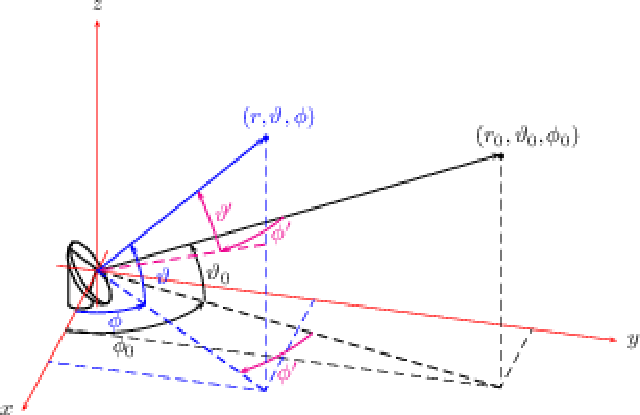
\includegraphics[width=0.7\textwidth]{\EPSDIR/schema-geometrie.pdf}
\caption{Spherical coordinates used to locate the target.}\label{coord-spher}
\end{figure}

When 
\begin{enumerate}
\item the resolution volume is small enough so that hydrometeor properties are uniform inside this volume,
\item the Rayleigh approximation is valid (wavelength much smaller than particle sizes),
\item scatterers are only made of liquid water,
\item attenuation is negligible,
\item the receiver's bandwidth is infinite,
\item the antenna's directivity function is  Gaussian,
\end{enumerate}
then (\ref{eqrad}) can be written as
\begin{equation}
P_r(\vec r_0)=C\frac{z(\vec r_0)}{r_0^2}\,,\label{eqradzC}
\end{equation}
where
\begin{equation}
z\equiv\int_0^\infty D^6N_r(D)d D\,,\label{eqray}
\end{equation}
is the \emph{radar reflectivity factor} and
\begin{equation}
C\equiv\frac{\pi^3 P_tg^2c\tau(\Delta\vartheta)^2|K_w|^2}{1024\lambda^2\ln2}
\end{equation}
is the \emph{radar constant}, where $c$ is the celerity of light in vacuum ($\rm m~s^{-1}$), $\tau$ is the pulse duration (s), $\Delta\vartheta$ is the beam width to the $-3\rm~dB$ level for one-way transmission ($\rm rad$), $|K_w|^2$ is the \emph{dielectric factor} for water (about $0.93$ for usual wavelengths). Under these assumptions, note that (\ref{eqray}) and (\ref{Zer}) are strictly identical (except that the units differ).

When the previous assumptions are not met, the radar measures \emph{equivalent reflectivity factors} which can be simulated by:
\begin{equation}
\bar z_e(\vec r_0)\equiv\frac{r_0^2P_r(\vec r_0)}C=\frac{16r_0^2\lambda^4\ln2}{\pi^6c\tau(\Delta\vartheta)^2|K_w|^2}\int_0^{2\pi}\!\!\!\int_0^\pi\!\!\!\int_0^\infty\frac{\eta(\vec r)l(\vec r)^2}{r^2}f^4(\vartheta',\phi')|W(r_0-r)|^2\sin\vartheta'd rd\vartheta'd\phi'\,.
\end{equation}


% Equivalent reflectivity factors are usually expressed in $\rm mm^6~m^{-3}$; in this case,
% \begin{equation}
% \bar z_e[{\rm mm^6~m^{-3}}]=10^{18}\bar z_e\,.
% \end{equation}
% Since the equivalent reflectivity factor takes values within several orders of magnitude, it is commonly expressed in dB$Z$:
% \begin{equation}
% \bar Z_e\equiv10\log\left(\frac{\bar z_e[\rm mm^6~m^{-3}]}{1~\rm mm^6~m^{-3}}\right)\,.
% \end{equation}
Since the equivalent reflectivity factor takes values within several orders of magnitude, it is commonly expressed in dB$Z$:
\begin{equation}
\bar Z_e\equiv10\log\left(10^{18}\bar z_e\right)\,.
\end{equation}

At present, the radar simulator does not take into account the finite bandwidth effect. So the expression used to compute reflectivities reads:
\begin{equation}
\bar z_e(\vec r_0)=\frac{8\lambda^4\ln2}{\pi^6(\Delta\vartheta)^2|K_w|^2}\int_0^{2\pi}\!\!\!\int_0^\pi\eta(\vec r)l(\vec r)^2f^4(\vartheta',\phi')\sin\vartheta'd\vartheta'd\phi'\,.\label{zefctradiale}
\end{equation}
The article by \citet{Caumont2006} summarizes this paragraph and provides an example of use of the reflectivity simulator on a case study.

With the same formalism as for reflectivity, Doppler velocity is expressed as follows:
\begin{equation}\label{vdopppi}
v_r(\vec r_0)=\frac{\displaystyle\int_0^{2\pi}\!\!\!\int_0^\pi\overline{\eta v_r}(\vec r)l(\vec r)^2f^4(\vartheta',\phi')\sin\vartheta'd\vartheta'd\phi'}{\displaystyle\int_0^{2\pi}\!\!\!\int_0^\pi\eta(\vec r)l(\vec r)^2f^4(\vartheta',\phi')\sin\vartheta'd\vartheta'd\phi'}\,,
\end{equation}
with
\begin{align}
\overline{\eta v_r}(\vec{r})&\equiv\sum_{j\in\rm type}\int_0^\infty\!\!\!\sigma_j(D,\vec{r})\left(u_r(\vec{r})-\sin\vartheta v_{T_j}(D,\vec{r})\right)N_j(D,\vec{r})d D\,,\\
&=\eta(\vec r)u_r(\vec{r})-\sin\vartheta\sum_{j\in\rm type}\int_0^\infty\!\!\!\sigma_j(D,\vec{r})v_{T_j}(D,\vec{r})N_j(D,\vec{r})d D\,,
\end{align}
where $u_r(\vec{r})$ is the projection onto the beam direction of the wind vector (in m~s$^{-1}$), and $v_{T_j}(D,\vec{r})$ is the fall speed of particles of diameter $D$ (in m) for the precipitating hydrometeor type $j$ (in m~s$^{-1}$).
More details about the simulation of Doppler velocities are provided by \citet{Caumont2008}. %\cite{cau08}.

A similar, yet more general expression than in the grid-point simulator (cf. (\ref{Z_{DR}})), is used to compute differential reflectivity (in dB) \citep[see][]{Seliga1976}: %\citep[see][]{sel76}:
\begin{equation}
Z_{DR}\equiv10\log\frac{z_{HH}}{z_{VV}}
\end{equation}
where $z_{HH}$ and $z_{VV}$ are equivalent reflectivity factors (in $\rm mm^6~m^{-3}$) at horizontal and vertical polarization, respectively.

Specific differential phase is computed from (\ref{DefKDP}) with a factor of $10^{3}$ to express it in $^\circ\rm~km^{-1}$.

Note that, as in the grid-point simulator, only raindrops contribute to $Z_{\it DR}$ and $K_{\it DP}$. Raindrops are considered as spheroids (when the scattering model allows for it; see below), the axis ratios of which are defined by (\ref{PB70}) or (\ref{ABL99}), as in the grid-point simulator.

\subsubsection{Numerical implementations}
\paragraph{Integrals over $D$.}
(\ref{eta}), (\ref{l}), (\ref{zefctradiale}), and (\ref{vdopppi}) contain improper integrals that cannot be directly computed. The angular double quadratures in (\ref{zefctradiale}) and (\ref{vdopppi}) are evaluated by following the method of \cite{Probert-Jones1962}, i.e., considering the antenna's radiation pattern as a Gaussian function, which means that only the main lobe is taken into account. Two similar techniques are implemented: Gauss-Hermite's and Gauss-Legendre's. In the following, $\eta(\vec r)l^2(\vec{r})$ or $\overline{\eta v_r}(\vec r)l(\vec r)^2$ are denoted as $F(\vec r)$.

\paragraph{Gauss-Hermite quadrature.} The first technique consists in approaching the bidimensional integral by two independent integrals over $]-\infty;\infty[$:
\begin{equation}
I=\int_0^{2\pi}\!\!\!\int_0^\pi f^4(\vartheta',\phi')F(\vec r)\sin\vartheta'd\vartheta'd\phi'=\int_{-\infty}^\infty\!\int_{-\infty}^\infty e^{-8\ln2\frac{\vartheta'^2}{\Delta\vartheta^2}}e^{-8\ln2\frac{\phi'^2}{\Delta\vartheta^2}}F(\vec r)d\vartheta'd\phi'\,.
\end{equation}
Then, the so-called Gauss-Hermite quadrature is used to evaluate the two improper integrals:
\begin{align}
I&\underset{\binom xy=\frac{\sqrt{8\ln2}}{\Delta\vartheta}\binom{\vartheta'}{\phi'}}=\frac{(\Delta\vartheta)^2}{8\ln2}\int_{-\infty}^\infty e^{-x^2}\!\int_{-\infty}^\infty e^{-y^2}F\left(r,\vartheta_0+\frac{x\Delta\vartheta}{\sqrt{8\ln2}},\phi_0+\frac{y\Delta\vartheta}{\sqrt{8\ln2}}\right)d yd x\,,\\
&\simeq\frac{(\Delta\vartheta)^2}{8\ln2}\sum_{i=0}^{n_H-1}\sum_{j=0}^{n_V-1}v_iw_jF\left(r,\vartheta_0+\frac{x_i\Delta\vartheta}{\sqrt{8\ln2}},\phi_0+\frac{y_j\Delta\vartheta}{\sqrt{8\ln2}}\right)\,,
\end{align}
where $x_i$ and $y_i$ are abscissas for the quadrature, $v_i$ and $w_i$ are the corresponding weights, and $n_H$ and $n_V$ are the corresponding numbers of abscissas. 


\paragraph{Gauss-Legendre quadrature.} The second technique consists in approaching the bidimensional integral by two independent integrals over $]-\Delta\vartheta/2;\Delta\vartheta/2[$:
\begin{align}
I&\simeq\int_{-\Delta\vartheta/2}^{\Delta\vartheta/2}\int_{-\Delta\vartheta/2}^{\Delta\vartheta/2}e^{-8\ln2\frac{\vartheta'^2}{\Delta\vartheta^2}}e^{-8\ln2\frac{\phi'^2}{\Delta\vartheta^2}}F(\vec r)d\vartheta'd\phi'\,,\\
&\underset{\binom xy=\frac{\Delta\theta}2\binom{\vartheta'}{\phi'}}\simeq\frac{(\Delta\theta)^2}4\int_{-1}^1 e^{-2\ln2x^2}\int_{-1}^1 e^{-2\ln2y^2}F\left(r,\theta_0+\frac{x\Delta\theta}2,\phi_0+\frac{y\Delta\theta}2\right)d yd x\,,\\
&\simeq\frac{(\Delta\theta)^2}4\sum_{i=0}^{n_H-1}\sum_{j=0}^{n_V-1}v_iw_j e^{-2\ln2x_i^2}e^{-2\ln2y_j^2}F\left(r,\vartheta_0+\frac{x_i\Delta\vartheta}2,\phi_0+\frac{y_j\Delta\vartheta}2\right)\,,
\end{align}
where $x_i$, $y_i$, $v_i$, $w_i$, $n_H$, and $n_V$ have similar roles as in the Gauss-Hermite quadrature, but correspond here to the Gauss-Legendre one.\\


The Gauss-Hermite quadrature is well-suited for low numbers of points (typically $\le3$), whereas the Gauss-Legendre quadrature is better suited for high number of points: above 3 points, the Gauss-Hermite quadrature evaluates the function in the integral for angles that are unrealistically far away from the direction of propagation, while under 3 points, the Gauss-Legendre quadrature does not provide consistent values, i.e., for $n_H=n_V=1$:
\begin{equation}
\frac{(\Delta\theta)^2}4v_0w_0 e^{-2\ln2x_0^2}e^{-2\ln2y_0^2}F\left(r_0,\theta_0,\phi_0\right)=(\Delta\theta)^2F\left(\vec r_0\right)\,
\end{equation}
which is different from $\frac{\pi(\Delta\theta)^2}{8\ln2}F\left(\vec r_0\right)\simeq0.567(\Delta\theta)^2F\left(\vec r_0\right)$ as would give a simple evaluation at the centre of the volume of resolution.\\


Similarly, the improper integral involving scatterer diameters is computed by using a Gauss-Laguerre quadrature. Further details concerning these quadrature techniques can be found in \citet{Press1992}. 


\paragraph{Scattering methods.}
Four methods are available: Rayleigh (for spheres), Mie, Rayleigh for spheroids and T-Matrix.

\begin{description}
\item {Rayleigh, Mie or Rayleigh for spheroids scattering methods}
  
The three first methods have been implemented and are described by \citet{Caumont2006}. 
When using Rayleigh, Mie or Rayleigh for spheroids methods,
hydrometeors containing ice are supposed to behave as isotropic scatterers as they fall or tumble (i.e., they are modeled as spheres).
The approximations of Rayleigh for spheres and for spheroids yield analytic results. Thus, for instance, in the Rayleigh theory, cross sections for raindrops are
\begin{align}
\sigma_{\rm HH}&=\frac{\pi^5|K_w^2|}{\lambda^4}D^6\,,\\
C_e&=\frac{\pi^2}\lambda\Im K_wD^3+\frac{\pi^4}{15\lambda^3}\Im\left(K_w^2\frac{m^4+27m^2+38}{2m^2+3}\right)D^5+\frac{2\pi^5}{3\lambda^4}\Re(K_w^2)D^6\,.
\end{align}
Analytic derivations of Rayleigh for spheroids cross sections can be found in \citet{Kerker1969} (Chap.~10), \citet{vandeHulst1981}, \citet{Doviak1993}, or \citet{Bringi2001}, for instance.
Mie computations rely on the code described by \citet{Bohren1983}. 

For pure water particles, the dielectric function is taken from \citet{Liebe1991}, while the model of \citet{Hufford1991} is taken for pure ice.  Here we make the following assumptions: for particles made of ice and air only (snow, primary ice, and graupel above the melting level), we consider the diameter of a sphere made of ice only that would have the same mass \citep[e.g.,][]{Smith1984}. For water-coated graupel, which are made of ice, water, and air, we consider the diameter of an equivalent-mass sphere made of 14~\% of water and 86~\% of ice as spheroidal inclusions \citep[following][]{Rasmussen1984}. The corresponding dielectric function is then computed following \citet{Bohren1982}.

\item{T-matrix scattering method}

When using T-matrix scattering method, implemented and described by \citet{Augros2016}, not only raindrops but also snow and graupel particles are considered as spheroids. 
The T-matrix code has been adapted from \citet{Mishchenko1998} and \citet{Mishchenko2002}. T-matrix lookup tables
containing the scattering coefficients were computed in advance
for each hydrometeor type and each radar wavelength (S, C and
X band). These coefficients were estimated for a set of diameters,
temperatures, elevation angles and liquid water fractions for
melting graupel. Polarimetric variables are calculated from the scattering coefficients following the equations given in the Appendix of \citet{Augros2016}.

When selecting T-matrix scattering method, a more continuous melting process is simulated for graupel particles. 
In a similar way to Jung et al (2008), the water
fraction inside graupel particles is estimated as a function of the hydrometeor contents of graupel and rain $M_g$ and $M_r$.
More details of this parameterization are explained by \citet{Augros2016}. 
\end{description}

\section{Satellite diagnostics}
A comparison between model outputs and satellite observations provides an assessment of how well the model can reproduce the meteorological situation.
 The model-to-satellite approach compares directly the satellite brightness temperatures (BTs) to the BTs computed from the predicted model fields 
\citep{Morcrette1991}. It has been first applied to Meso-NH outputs for comparison
 with Meteosat observations in the infrared using a narrow-band code 
\citep{Chaboureau2000}, then for the tuning of a critical parameter in the microphysical scheme \citep{Chaboureau2002a}.

Since the Masdev 4-7 version, the Radiative Transfer for Tiros Operational Vertical Sounder (RTTOV) code version 11.3 \citep{Saunders2005} is also available
allowing the calculation of BT for a large number of satellites. RTTOV was first used with Meso-NH for a further tuning in the microphysical scheme \citep{Chaboureau2006}. The paragraphs below are taken from the RTTOV documentation. They give a broad overview on the RTTOV model. More information can be obtained from the web ressources on {\tt https://nwpsaf.eu/site/software/rttov/ }

The RTTOV model allows rapid simulations of radiances for satellite infrared or
microwave nadir scanning radiometers given an atmospheric profile of
temperature, variable gas concentrations, cloud and surface properties.
Ozone and carbon dioxide are taken from the \citet{McClatchey1972} standard
profiles and the fixed value used in Meso-NH, respectively. Above the model
top, the standard profiles from \citet{McClatchey1972} are used.
All the atmospheric profiles of temperature and gas concentrations are then
interpolated onto the 43 pressure levels of RTTOV.

Currently the spectral range of the RTTOV model is 3-20 $\mu$m (500-3000
cm$^{-1}$)  in the infrared governed by the range of the GENLN2
line-by-line dataset on which it is based.
In the microwave the frequency range from 10-200 GHz is covered using
the Liebe-89 MPM line-by-line model. The full list of currently
supported platforms and sensors is given in Tables 2 and 3 of
the RTTOV users guide (and duplicated on the Meso-NH users guide).
Simulation of clear radiances are based on transmittances computed by means
of a linear regression in optical depth.

In the infrared, the RTTOV code takes clouds into account as grey bodies
\citep{Chevallier2001} on the Meso-NH defined model level assuming
maximum random overlap of clouds. Radiative properties for water clouds
are calculated using constants tabulated in \citet{Hu1993}.
Water cloud effective radius is diagnosed using a value of 10 $\mu$m
over land and 13 $\mu$m over sea.
Radiative properties for ice clouds are taken from \citet{Baran2004}
assuming hexagonal columns with an effective dimension diagnosed
from the ice water content \citep{McFarquhar2003}.
Surface emissivity is given by the Ecoclimap database \citep{Masson2003}.
Note that the surface emissivity is valid there for a broad band
between 8 and 12 $\mu$m only.

In the microwaves, the hydrometeor optical properties are provided to the RTTOV
model from precomputed Mie tables for liquid water, cloud ice, rain, and
precipitating ice \citep{Bauer2001}. The cloud layers are overlapped following
a maximum random approximation. Polarization is only introduced by the sea
surface properties obtained using the FASTEM code. Elsewhere (over land
and sea-ice) surface emissivity is fixed with typical value of bare soil.


%%%%%%%%%%%%%%%%%%%%%%%%%%%% BIBLIOGRAPHY %%%%%%%%%%%%%%%%%%%%%%%%
\begin{btSect}{5-2-Diagnostics}
\section{References}
\btPrintCited
\end{btSect}
%%%%%%%%%%%%%%%%%%%%%%%%%%%% BIBLIOGRAPHY %%%%%%%%%%%%%%%%%%%%%%%%
